\documentclass[12pt,a4paper,oneside]{article}
\usepackage[english]{babel}
\usepackage{amsmath}
\usepackage{amsfonts}
\usepackage{amssymb}
\usepackage{natbib}
\usepackage{float}
\usepackage{url}
\usepackage[pdftex]{graphicx}
\usepackage[left=1in,right=1in,top=1in,bottom=1in]{geometry}
\author{Pieter Verlinden}
\title{Assignment2}

\begin{document}
\begin{titlepage}
\begin{center}

\includegraphics[scale=0.25]{logo.jpg} \\
%
\includegraphics[scale=width=0.15\textwidth]{.logo.jpg}\\[1cm]
\textsc{\large Katholieke Universiteit Leuven}\\[4cm]
\textsc{\LARGE Data Structures and Algorithms}\\[0.5cm]
\newcommand{\HRule}{\rule{\linewidth}{0.5mm}}
% Title
\HRule \\[0.5cm]
{ \huge \bfseries Assignment 2 \\ \large{ 8-Puzzle }}\\[0.5cm]

\HRule \\[1.5cm]

%Author and lecturer
\begin{minipage}{0.45\textwidth}
\begin{flushleft} \large
\emph{Author:}
Pieter \textsc{Verlinden}\\

\emph{Student ID:}
r0369547\\

\emph{Study:}
1Ba Informatica

\end{flushleft}

\end{minipage}
\hfill
\begin{minipage}{0.45\textwidth}
\begin{flushleft} \large
\emph{Lecturer:} 
Dr.~Ir.~Philip \textsc{Dutr\'{e}}
\end{flushleft}
\end{minipage}

\vfill

%bottom
{\large April 5, 2013}

\end{center}
\end{titlepage}
\tableofcontents
\newpage
\section{Introduction}
The purpose of this assignment is to study the importance of data-structures, in particular the "priority-queue", by writing a program that solves the 8-puzzle-problem (see section \ref{sec:8puz}). 
\\

This puzzle-problem can be solved by implementing the A* algorithm\cite{A*Wiki}. This algorithm uses priorityfunctions such as the Manhatten priority and the Hamming priority (see section \ref{sec:solveA*}), to determine the closest path to the goalstate.
\\

In section \ref{sec:expData}, some experimental data will be given based on the two used priorityfunctions. With this data, conclusions will be made and some questions will be answered in section \ref{sec:CoClar}.
\newpage

\section{8-puzzle}\label{sec:8puz}
The 8-puzzle, also called a sliding puzzle, is a puzzle that consists of a frame of numbered tiles in random order (see Figure \ref{fig:8-puz}).
\begin{figure}[H]
	\centering
	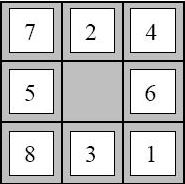
\includegraphics[scale=0.85]{8-puz.jpg} 
	\caption{An unsolved 8-puzzle.}
	\label{fig:8-puz}
\end{figure}

\subsection{Solvemethod - A* algorithm}\label{sec:solveA*}
To solve this kind of puzzles, we use the widely known "A* algorithm"\cite{A*Wiki} developed by Peter Hart, Nils Nilsson and Bertram Raphael.\\
To implement this algorithm, we first define a state. This state holds the number of moves made so far, the current board position (the configuration of the board) and the previous state.\\
Each initial board has neighbours (a.k.a. all the boards with swapped empty places). Create a state of each neighbour and add it to a minimum priority queue. Delete and assign the state with the least priority to a temporary state, and repeat the above algorithm.\\

The priority of each state is the key to success of this algorithm. Two priorityfunctions are defined: the Manhattan priorityfunction and the Hamming priorityfunction.\\
The Manhattan priorityfunction holds the sum of the distances between the position of each element and its goalposition. The Hamming priorityfunction holds the amount of elements out of place\cite{princetonPuzzle}.\\

By taking the state with the least priorityscore (a.k.a. the board with the least distance between this state an the goalstate or the amount of tiles out of place) we know that this state is closest to the goalstate.
\subsection{Experimental data}\label{sec:expData}
\begin{table}[H]
\centering
\begin{tabular}{ l | l | l | l }
	puzzle & moves & Hamming (s) & Manhattan (s) \\ \hline
	puzzle28.txt & 28 & 2 & 1  \\
	puzzle30.txt & 30 & 4 & 1  \\
	puzzle32.txt & 32 & \textgreater 5min & 2 \\
	puzzle34.txt & 34 & \textgreater 5min & 1 \\
	puzzle36.txt & 36 & \textgreater 5min & 4 \\
	puzzle38.txt & 38 & \textgreater 5min & 4 \\
	puzzle40.txt & 40 & \textgreater 5min & 2 \\
	puzzle42.txt & 42 & \textgreater 5min & 8 \\ \hline	
\end{tabular}
	\caption{Experimental data on the A* algorithm for solving 8-puzzles.}
	\label{tab:expData}
\end{table}

From this data we can conclude that the Manhattan priorityfunction is extensively more efficient than the Hamming priority. This is due to the fact that the Hamming priority gives less information about the configuration of a board than the Manhattan priority.
\newpage
\section{Code clarification}\label{sec:CoClar}
In this section, some of the implemented code will be clarified and explained.\\

Board.java first constructs a board of tiles, using a two-dimensional array. Then, it stores the indexes of the empty spot in two variables. The class also implements the Iterable interface, which makes it possible to loop through all the neighbouring boards of this board.\\
Neighbours are boards with a tile configuration where the empty spot is moved one tile from its initial spot, in each direction (see Figure \ref{fig:8-puz_neighbours}).
\begin{figure}[H]
	\centering
	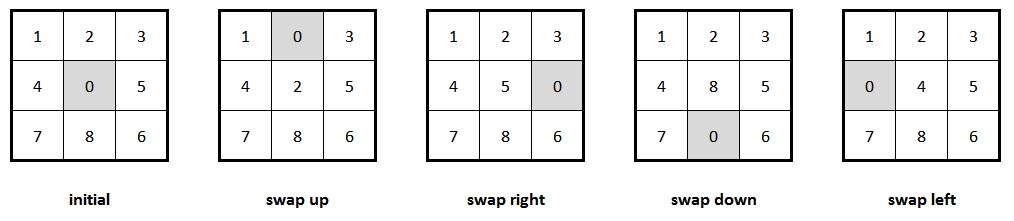
\includegraphics[scale=0.75]{8-puz_neighbours.jpg} 
	\caption{An initial 8-puzzle board and its neighbours.}
	\label{fig:8-puz_neighbours}
\end{figure}

To get these neighbouring boards, extra methods such as "swapUp" and "swapLeft" and extra checkers such as "isSwappableUp" and "isSwappableLeft" are made. These functions use a new exchange method that swaps elements in a two-dimensional array.\\

A state (as explained in section \ref{sec:solveA*})is defined by implementing a new class: InterState.java. This class implements the interface Comparable, which makes it possible to put InterState objects in a priority queue. On top of that, it holds an integer "moves" which holds the current amount of moves done so far, a previous InterState, the current board and finally an integer holding the priorityscore. This score consists out of the sum of the amount of moves and an amount of a priorityfunction. \\

To check whether a puzzle is solvable, an isSolvable method is made in Solver.java. This method is slightly different from the given method, and is based on the method of odd and even inversions stated in the 8 puzzle assignment: cos 226 from Princeton University\cite{princetonPuzzle}.

From the experimental data (see Table \ref{tab:expData}), we can derive that the priorityfunction is a key element to a good and fast working algorithm. The Manhattan priorityfunction is significantly faster and less memory-absorbent than the Hamming priorityfunction. So if we ask ourselves, what is the best solution for bigger and more difficult puzzles, we could answer that a thorough study on priorityfunctions is the most efficient way to fasten our algorithm. If this is still not enough, more memory could be added. The law of Moore\citep{MooreLaw} states that transistors on integrated circuits, double every eighteen months. This makes enlarging the memory a plausible solution. 
\newpage

\section{Conclusion}
In my opinion, this assignment was very instructive and informative. It shows us that a good algorithm can solve almost any problem in a significant amount of time. By implementing the famous A* algorithm, I acquired more insight in the solving of problems and more experience in debugging and optimizing my code.
Also concepts like a priority queue, interfaces and generic types like Iterable and Comparable are more clear to me now. \\
Though this assignment costed a lot of time and work, the experience and knowledge gained was fully worth it.
\newpage
\bibliographystyle{plain}
\bibliography{ref}
\end{document}